\subsection{Kanter}\label{subsec:kant}
Hvis et billede beskues i 3D, som en figur, hvor hver pixel har een intensitet, kan en kant illustreres i 1D , ved et snit af et billede vinkelret på overfladen, som ses på figur \ref{fig:kant}. En kurve, angiver et intensitetsskift.
\noindent
\begin{figure}[H]
    \centering
    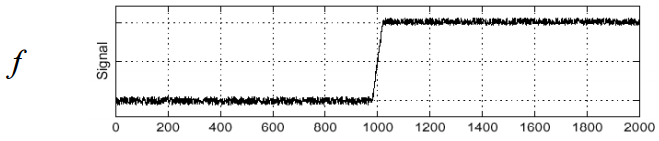
\includegraphics[width=0.55\textwidth]{fig/7.png}
     \vspace{-1em}
    \begin{center}        
     \caption{\textcolor{gray}{\footnotesize \textit{
     En 1-dimensional fortolkning af intensiteten i et billede. De små udsving indikere støj, den store kurve repræsenter et skift i intensiteten og derved en kant i et billedet.}}}
    \label{fig:kant}
     \end{center}
       \vspace{-2.5em}
  \end{figure}
\noindent
En differentiering af funktionen fra figur \ref{fig:kant} vil angive, hvor skarp kurven er og derved fremhæve dens udsving. Et billede i 2D er ikke en kontinuerlig funktion, men består af diskrete værdier i form af pixel informationer.
Differentiering af billeder sker der approsikmeret: \begin{equation}
\dfrac{df(x)}{dx}=\dfrac{f(x+1)-f(x-1)}{2}
\label{diff}
\end{equation}
ligning \eqref{diff} kan udføres på billedet ved at folde billedet med kernen $[\frac{1}{2} \hspace{0.3cm} 0 \hspace{0.3cm} -\frac{1}{2}]$. 
\\
\\
Som det senere vil beskrives, er foldning af et billede nyttigt i flere tilfælde: Bl.a. når der skal differentieres:
\\
Foldning af $I$ med af størrelse $(M \times N)$, med en kerne $K$ med størrelse $(m \times n)$, hvor $M > k, N > n$, defineres ved:
\begin{equation}
O(i,j) = \sum\limits_{k=1}^m \sum\limits_{l=1}^n I(i+k-1,l-1)K(k,l)
\end{equation}
\\
og udføres af operatoren: $\times$. \\
I tilfælde af, at en kerne skal foldes med et område i billedet, der rækker udover billedet, er det i denne opgave vedtaget, at dette område får billedværdi($I$) 0. Eg. $O(1,1)$, med er kerne der har størrelse $M > m > 1$, $N > n > 1$, vil værdien af $I(i+k-1 < 0, l-1 <0) = 0$  \\
\\
Problemet ved differentiering, visualiseret i figur \ref{fig:kant}, er at støj i billedet (de små udsving) også vil blive fremhævet, hvilket kan resultere i fejlagtige detektioner af kanter. For at fjerne støjen foldes billedet med et Gaussisk filter, hvilket er en diskret approksimering til den Gaussiske funktion. Foldning af et billede med et Gaussisk filter vil resultere i en "flydende" overgang mellem pixel værdierne og derfor glatte billedet. Den Gaussiske funktion i 2-D, hvor $ \sigma $ er standardafvigelsen af den Gaussiske fordelingen, er defineret som:
\begin{equation}
G(x,y,\sigma) = \frac{1}{2 \pi \sigma ^{2}} e^{- \frac{x^{2} + y^{2}}{2 \sigma ^{2}}}
\label{2dgaussian}
\end{equation} 
For at undgå to itereration af foldning for differentiering og sløring, kan dette udføres i en samlet operation, ved at folde billedet med et differentieret Gaussisk filter, da foldning er en associativ operation.
\begin{equation}
\dfrac{\partial}{\partial x}(G \ast f) = (\dfrac{\partial}{\partial x}G) \ast f
\end{equation}
Foldes et 1 dimensionelt gaussfilter med kanten \ref{fig:kant}, vil det resultere i et bakkeformet signal, hvor bakken indikere en kant. For en mere lokaliserbar kant, kan den dobbelt afledte tages, som set i figur \ref{fig:deriv}.
\begin{figure}[H]
    \centering
    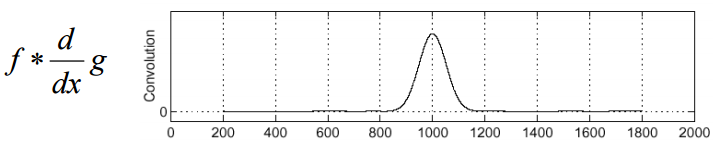
\includegraphics[width=0.55\textwidth]{fig/8.png}
    \vspace{-1em}   
    \begin{center}
    \caption{\textcolor{gray}{\footnotesize \textit{
     Resultatet af at folde et dobbelt differentieret Gaussisk filter med funktionen}}}
    \label{fig:deriv}
     \end{center}
    \vspace{-2.5em}  
  \end{figure}
\noindent
Kanten kan nu lokaliseres, ved funktionens krydsning af 0.